\documentclass[12pt,a4paper,oneside,final,titlepage,openany,onecolumn]{article}
\usepackage[latin1]{inputenc}
\usepackage{amsmath}
\usepackage{amsfonts}
\usepackage{amssymb}
\usepackage{graphicx}
\usepackage{listings, lstautogobble}
\usepackage{xcolor}
\usepackage{float}
\usepackage{changepage}

\lstset{ %
	backgroundcolor=\color{gray!10!white},   % choose the background color; you must add \usepackage{color} or \usepackage{xcolor}; should come as last argument
	basicstyle=\footnotesize\ttfamily,        % the size of the fonts that are used for the code
	breakatwhitespace=false,         % sets if automatic breaks should only happen at whitespace
	breaklines=true,                 % sets automatic line breaking
	captionpos=b,                    % sets the caption-position to bottom
	commentstyle=\color{green!50!black},    % comment style
	morecomment=[l]{\%},
	deletekeywords={},            % if you want to delete keywords from the given language
	escapeinside={*@}{@*},          % if you want to add LaTeX within your code
	extendedchars=true,              % lets you use non-ASCII characters; for 8-bits encodings only, does not work with UTF-8
	%frame=single,                    % adds a frame around the code
	keepspaces=true,                 % keeps spaces in text, useful for keeping indentation of code (possibly needs columns=flexible)
	keywordstyle=\color{blue},       % keyword style
	%language=Matlab,                 % the language of the code
	morekeywords={for, end, if},            % if you want to add more keywords to the set
	numbers=left,                    % where to put the line-numbers; possible values are (none, left, right)
	numbersep=5pt,                   % how far the line-numbers are from the code
	numberstyle=\tiny\color{gray}, % the style that is used for the line-numbers
	rulecolor=\color{black},         % if not set, the frame-color may be changed on line-breaks within not-black text (e.g. comments (green here))
	showspaces=false,                % show spaces everywhere adding particular underscores; it overrides 'showstringspaces'
	showstringspaces=false,          % underline spaces within strings only
	showtabs=false,                  % show tabs within strings adding particular underscores
	stepnumber=1,                    % the step between two line-numbers. If it's 1, each line will be numbered
	stringstyle=\color{green!30!black},     % string literal style
	tabsize=2,                    % sets default tabsize to 2 spaces
	autogobble=true,      %align left
	%fontname=\ttfamily
}


\author{Giacomo Deodato\\ Alessandro Patti}
\title{Image Processing\\ \textbf{Report on Laboratory Session \#5}}
\date{November 13, 2017}
\pagenumbering{gobble}
\usepackage{ragged2e}
\widowpenalty 10000

\begin{document}
	\maketitle
	\section*{{\small Part \#1} \\ Processing of stereo images. Stereo matching}
		\par
		For the first part of the exercise we completed the \textit{Matching()} function so that it can correctly compute the Sum of Absolute intensity Differences and then fill the disparity map with the shift leading to the minimum SAD.
		\begin{lstlisting}
			% compute Cost from Sum absolute Diffrences(SAD)
			for c=1:1:P
				SAD=SAD+abs(imL(i+k,j+l,c)-imR(i+k,j+l-d,c));
			end
		\end{lstlisting}
		\begin{lstlisting}
			%to change disp to d value  having the least dissimilarity
			if (SAD<error)
				error = SAD;
				disp(i,j) = d;
			end 
		\end{lstlisting}
		\par
		Then we read the source images and we computed the disparity map using the matching function with given parameters (dmax = 45, and block size of 3 and 9).
		\begin{figure}[h!]
			\centering
			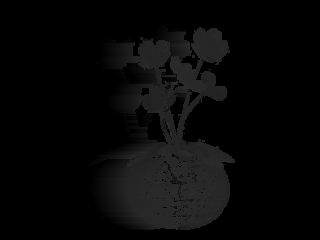
\includegraphics[width=0.8\linewidth]{images/disp_map2_01_3.png}
			\caption{Disparity map with block size of 3.}
		\end{figure}
		\begin{figure}[h!]
			\centering
			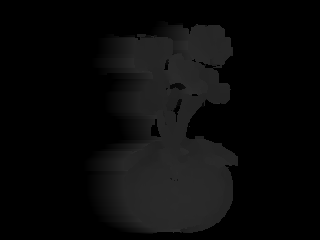
\includegraphics[width=0.8\linewidth]{images/disp_map2_01_9.png}
			\caption{Disparity map with block size of 9.}
		\end{figure}
		\par
		It can be noticed that increasing the block size produces less noisy results because the matching function has better precision when comparing bigger blocks of pixels but this comes with an increase in the computation cost (for the same reason we already scaled the image by a factor of 0.4).
		\newline
		\par
		To reduce the noise in the first disparity map an average filter with kernel size of 3 has been used.
		\newline
		\par
		Finally we applied the matching process also to the other couples of images with block size of 1, from the results we can see that as the baseline increases we obtain separated figures inside the same map, also due to the distance values and the block size.
		
	\section*{{\small Part \#2} \\ Processing of stereo images. Depth computation and segmentation}
		\par
		For this exercise we started by completing the code of the \textit{DepthCompute()} function respecting the following equation:
		\[Z(x, y) = f\cdot\dfrac{B}{disp(x, y)},\quad for\ disp(x, y) \neq 0\]
		\[Z(x, y) = 255,\quad for\ disp(x, y) = 0 \]
		\begin{lstlisting}
			function [ DepthMap] = DepthCompute (disp, B, f )
				[N, M] = size(disp);
				DepthMap = zeros(N,M);
				max = 255;
				
				for i = 1:1:N
					for j = 1:1:M
						if (disp(i,j) == 0)
							DepthMap(i, j) = max;
						else
							DepthMap(i,j) = f * B / disp(i, j);
						end
					end
				end
		\end{lstlisting}
		Then we created the ex2 file, we read the source disparity map and converted it to depth map by means of \textit{DepthCompute()}.
		\newline
		\par
		To obtain a smoother result we applied median filtering with kernel size of 19 to the resulting image.
		\newline
		\par
		Finally we read the left image of the stereo pair, warped it on the depth data, and showed the results.
		\begin{lstlisting}
		figure;
		warp(-depth_map_filtered, imgL);
		title("Warp of the image on the stereo data. Hit ENTER to change view.");
		rotate3d on
		view([0,90]);
		pause;
		view([0,0]);
		pause;
		view([60,60]);
		pause;
		\end{lstlisting}
		\par
		The second part of the exercise required to separate the background and the different planes in the foreground.
		\newline
		In order to do that we displayed the histogram of the distribution of grey values in the depth map and we took 1 user input to separate background and foreground and 2 user inputs to separate three layers on the foreground.
		\newline
		To obtain the final RGB image we created a 3D matrix with 3 layers to separate the Red, Green and Blue channels, then we assigned the correct values to the pixel indexed by the \textit{find()} function.
		\newpage
		\begin{lstlisting}
		% Show distribution of the values.
		figure;
		imhist(uint8(depth_map_filtered));
		title('Distribution of grey values in the depth map')
		
		% Subtract the background
		x = ginput(1);
		background = find(depth_map_filtered > x(1));
		depth_map_filtered(background) = 255;
		depth_map_filtered = 255-depth_map_filtered;
		figure;
		imshow(uint8(depth_map_filtered),[]);
		title("Background subtraction");
		
		% Separate intermediate layers and foreground
		figure;
		imhist(uint8(depth_map_filtered));
		title('Identify to thesholds *@for@* intermediate planes');
		x = ginput(2);
		if x(1) > x(2)
			tmp = x(1);
			x(1) = x(2);
			x(2) = tmp;
		end
		[N, M] = size(depth_map_filtered);
		rgb_map = zeros([N M 3]);
		
		[row, col] = find(depth_map_filtered < x(1) & depth_map_filtered > 0);
		for i = 1:size(row)
			rgb_map(row(i), col(i), 1) = 255;
		end
		[row, col] = find(depth_map_filtered < x(2) & depth_map_filtered > x(1));
		for i = 1:size(row)
			rgb_map(row(i), col(i), 2) = 255;
		end
		[row, col] = find(depth_map_filtered > x(2));
		for i = 1:size(row)
			rgb_map(row(i), col(i), 3) = 255;
		end
		imshow(rgb_map);
		\end{lstlisting}	
	\section*{{\small Part \#3} \\ 3D displays using colour filter glasses. Anaglyph producing and perceiving in 3D}
		\par
		For the last exercise we just uploaded the two source images, created a new image with same dimensions and copied the red channel of the left image and the green and blue channels of the right one.
		\newline
		Finally we showed the result of this exercise and the "Lion Statue anaglyph" image to look at them with colour filter glasses.
		\begin{lstlisting}
			% read source images
			img0 = imread('Pair_anaglyph/x=0.0.jpg');
			img1 = imread('Pair_anaglyph/x=0.1.jpg');
			
			% copy the red color channel of the left image
			img(:,:,1)=img0(:,:,1);
			
			% copy the green and blue channels of the right image
			img(:,:,2)=img1(:,:,2);
			img(:,:,3)=img1(:,:,3);
			
			% show the result
			figure;
			imshow(img);
			title('Flower Anaglyph');
			
			% show the lion statue anaglyph
			figure;
			imshow(imread('Lion_anaglyph/Lion_Statue_anaglyph.jpg'));
			title('Lion statue anaglyph');
		\end{lstlisting}
	
\end{document}